\section{Basics}


\subsection{Poisson Reconstruction Overview}

Kazhdan, Bolitho and Hoppe described in \cite{Kazhdan06}
the Poisson Surface Reconstruction algorithm.
CGAL implements a variant of this algorithm which computes an implicit function
piecewise-linear in a 3D Delaunay triangulation instead of an octree.

The outline of this algorithm is:

\begin{enumerate}
\item Input is a 3D point set with oriented normals.
\item Build Delaunay triangulation.
\item Delaunay refinement (break bad tetrahedra, where {}``bad'' means
badly shaped or too big). The normal of Steiner points is set to zero.
\item Compute an indicator function f() piecewise-linear over the tetrahedra.
We solve the Poisson equation Laplacian(f) = divergent(normals field)
at each vertex of the triangulation via the TAUCS sparse linear solver.
\item CGAL Surface Mesh Generator extracts the iso-surface {}``f() = median
of f() over the input points''.
\end{enumerate}

% Insert image poisson.jpg/eps
\begin{center}
    \label{Surface_reconstruction_3-fig-poisson}
    % Image
    \begin{ccTexOnly}
        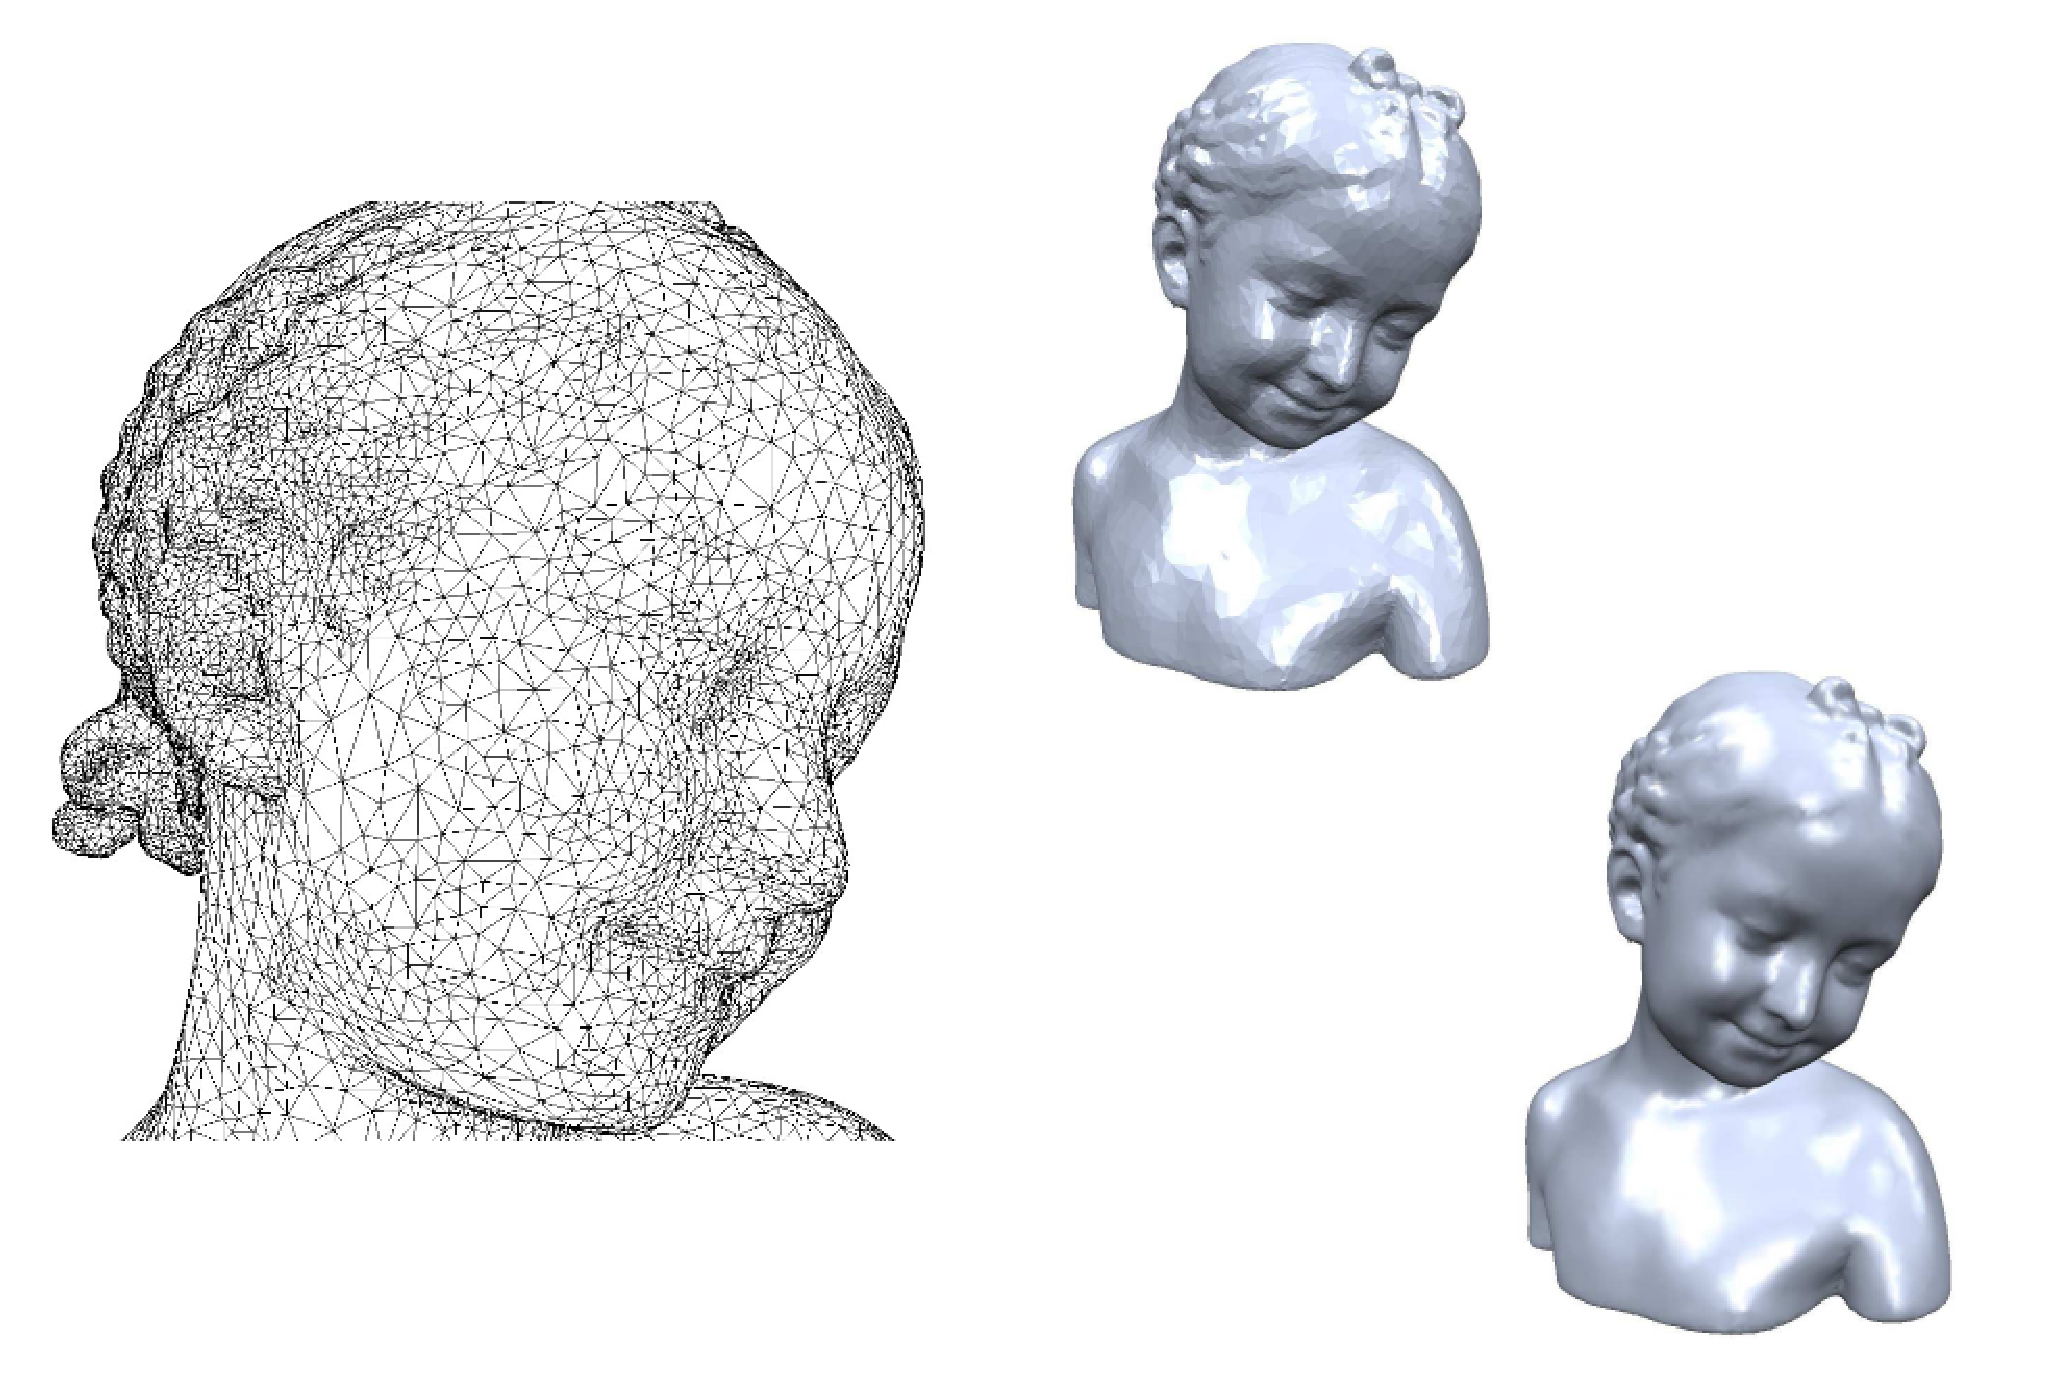
\includegraphics[width=0.9\textwidth]{Surface_reconstruction_3/poisson} % omit .eps suffix
    \end{ccTexOnly}
    \begin{ccHtmlOnly}
        <img width="90%" border=0 src="./poisson.jpg"><P>
    \end{ccHtmlOnly}
    % Title
    \begin{figure}[h]
        \caption{Poisson reconstruction of the Bimba point set (from scanner)}
    \end{figure}
\end{center}


\subsection{Poisson Reconstruction Example}

\ccc{poisson_reconstruction.cpp} reads a point set, creates a Poisson implicit function,
extracts the surface and saves it.

\ccIncludeExampleCode{Surface_reconstruction_3/poisson_reconstruction.cpp}


